\chapter{T 對偶、D 膜與規範理論}

\lectureoverview{T 對偶最初是半徑為 (R) 的圓上的閉弦，與半徑為 \(\alpha'/R\) 的圓上的閉弦之間的精確等價。動量與纏繞互換角色，世界面導數 \(\partial_\tau Y\) 與 \(\partial_\sigma Y\) 也互換，而由 \(G_{\mu 5}\) 與 \(B_{\mu 5}\) 降維而來的時空向量亦然。對開弦施行相同的操作時，Neumann 端點條件會變成 Dirichlet 條件。於是端點必須位於一個具有動力學的 D 膜上。受限於單一膜上的開弦，在低能下產生阿貝爾規範理論；連接一疊膜的弦帶有兩個端點標記，並產生非阿貝爾規範理論。終止於 D3 膜上的 D 弦，則提供相應的磁單極子。}

\section{為什麼要回到 T 對偶？}

我們先前已經談過 T 對偶，但現在再次討論它自有原因。它是弦理論所蘊含的遠不止微擾弦的一項線索。理解 T 對偶對開弦的影響後，便導出了 D 膜；D 膜又成為建構和研究量子場論的一種方法。因此，本講的目的不只是重述「小圓等價於大圓」這句口號。我們會仔細重建論證，藉此看出這句口號如何迫使理論納入新的物理物件。

最簡單的情況是環面緊緻化。一維環面就是圓。二維環面可表示為一個對邊互相識別的平行四邊形，三維環面則可表示為一個對面互相識別的平行六面體。同樣的構造可以延伸到更高維。我們只保留一個緊緻空間座標，稱為 \(Y\)，以及一個代表性的非緊緻座標，稱為 \(X\)。時間也在其中，只是不畫在板書圖上。

採用標準約定
\begin{equation}
  Y\sim Y+2\pi R,
  \label{eq:l10-circle-identification}
\end{equation}
使 \(R\) 表示半徑，\(2\pi R\) 表示圓周長。本講常將緊緻方向的尺度簡稱為 \(r\)，並略去 \(2\pi\) 與 \(\alpha'\) 的因子。我們會在推導中保留慣用因子，並在適當之處列出本講使用的單位。

討論的前半段探討的是有向閉弦。取向是沿弦畫出的內在箭頭。若將所有箭頭一律反向，任何實驗結果都不會改變；重要的是兩根弦之間的相對取向。弦分裂與合併時，箭頭必須連續銜接。這是帶符號的守恆量即將出現的第一個跡象。

\begin{figure}[H]
  \centering
  \includegraphics[width=0.72\textwidth]{lecture_10_figure_01.png}
  \caption{板書標出了兩根閉弦及其相對取向。分裂與合併的過程中，取向必須保持連續。}
  \lectureframe{00:05:40}
  \label{fig:l10-oriented-closed-strings}
\end{figure}

\begin{classroomqa}
\audiencequestion{如果世界面座標從 \(\sigma=0\) 走到 \(2\pi\)，弦是否已經繞緊緻方向一圈？\lecturetimestamp{00:08:42}}
\lecturerresponse{沒有。座標 \(\sigma\) 標記的是弦上的點，而不是緊緻空間中的位置。每根閉弦都有週期參數 \(\sigma\)，不論它是否纏繞。橡皮筋的比喻很有用：即使橡皮筋沒有繞在任何東西上，也可以沿著橡皮筋為分子編號。纏繞是映射 \(Y(\tau,\sigma)\) 的性質，不能只由參數 \(\sigma\) 決定。}
\end{classroomqa}

\begin{classroomqa}
\audiencequestion{緊緻方向的尺度是否也必須在大尺度座標 \(X\) 的每個位置都相同？\lecturetimestamp{00:10:00}}
\lecturerresponse{一般的動力學緊緻化不必如此。我們先從固定的圓開始，因為這是最簡單明瞭的背景。之後，分量 \(G_{55}\) 會成為一個標量場，其數值代表第五方向的局部尺度，因此這個尺度可以在普通時空中變化。}
\end{classroomqa}

\section{弦重新接合時，纏繞數仍然守恆}

未纏繞的弦可以沿緊緻方向移動，卻不繞行該方向。纏繞的弦則不同：當 \(\sigma\) 沿閉弦走一圈時，嵌入映射 \(Y(\tau,\sigma)\) 會在緊緻圓上前進一個或多個週期。弦具有取向，因此這段位移帶有正負號；弦可以沿正方向或負方向纏繞。

從弦接合的圖示最容易看出守恆定律。取一根纏繞數為 \(+1\) 的弦，以及另一根纏繞數為 \(-1\) 的弦。兩者方向相容的部分可以重新接合。所得組態的淨纏繞數為零，並且可以形變成一根未纏繞的弦。板書描繪的正是這種取向相反的重新接合。

\begin{figure}[H]
  \centering
  \includegraphics[width=0.72\textwidth]{lecture_10_figure_02.png}
  \medskip

  \begin{tikzpicture}[x=1cm,y=1cm,>=Latex]
    \draw[thick] (-4.0,0.3) circle (0.65);
    \draw[->,thick] (-4.55,0.58) arc (150:-145:0.65);
    \node at (-4.0,-0.65) {$w=+1$};
    \draw[thick] (-2.0,0.3) circle (0.65);
    \draw[<-,thick] (-2.55,0.58) arc (150:-145:0.65);
    \node at (-2.0,-0.65) {$w=-1$};
    \node at (-3.0,0.3) {$+$};
    \draw[->,thick] (-1.0,0.3) -- (0.3,0.3);
    \draw[thick] (1.4,0.3) ellipse (0.95 and 0.55);
    \node at (1.4,-0.65) {$w_{\rm total}=0$};
  \end{tikzpicture}
  \caption{纏繞方向相反的弦重新接合後，形成淨纏繞數為零的組態。下圖是對板書操作的清楚重建，並非另一個動力學過程。}
  \lectureframe{00:13:20}
  \label{fig:l10-opposite-winding}
\end{figure}

現在以兩根取向相同的弦重做這個過程。它們可以接合，但無法解除纏繞。所得弦的纏繞數是任一入射弦的兩倍。連通弦的數目變了，總纏繞數卻沒有改變。

\begin{figure}[H]
  \centering
  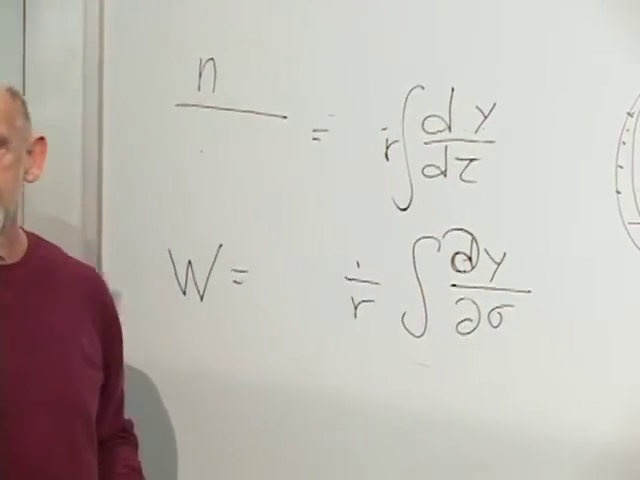
\includegraphics[width=0.72\textwidth]{lecture_10_figure_03.png}
  \medskip

  \begin{tikzpicture}[x=1cm,y=1cm,>=Latex]
    \draw[thick] (-4.0,0.3) circle (0.65);
    \draw[->,thick] (-4.55,0.58) arc (150:-145:0.65);
    \node at (-4.0,-0.65) {$w=+1$};
    \draw[thick] (-2.0,0.3) circle (0.65);
    \draw[->,thick] (-2.55,0.58) arc (150:-145:0.65);
    \node at (-2.0,-0.65) {$w=+1$};
    \node at (-3.0,0.3) {$+$};
    \draw[->,thick] (-1.0,0.3) -- (0.3,0.3);
    \draw[thick] (1.45,0.3) circle (0.78);
    \draw[thick] (1.45,0.3) circle (0.52);
    \draw[->,thick] (0.81,0.74) arc (145:-145:0.78);
    \node at (1.45,-0.78) {$w=+2$};
  \end{tikzpicture}
  \caption{纏繞方向相同的弦可以重新接合，形成纏繞兩次的弦。連通性雖有改變，總纏繞數仍為二。}
  \lectureframe{00:16:40}
  \label{fig:l10-same-winding}
\end{figure}

這項區別在所有允許的過程中都成立。總纏繞數為一百，可以由一根纏繞一百次的弦承載，也可以由兩根各纏繞五十次的弦，或一百根各纏繞一次的弦承載。弦可以在這些情況之間分裂與接合，但帶符號的總和始終是一百。我們以 \(w\in\mathbb Z\) 表示。

\section{動量模態與纏繞模態}

光有守恆還不足以構成對偶性。接下來要比較能量。沿緊緻圓方向運動的態具有量子化動量
\begin{equation}
  p_Y=\frac{n}{R},
  \qquad n\in\mathbb Z.
  \label{eq:l10-compact-momentum}
\end{equation}
若可忽略該態的其他質量貢獻，緊緻方向的運動會貢獻 \(E_{\rm mom}=|n|/R\)。正、負的 \(n\) 代表相反的運動方向，但能量仍為正。

\begin{figure}[H]
  \centering
  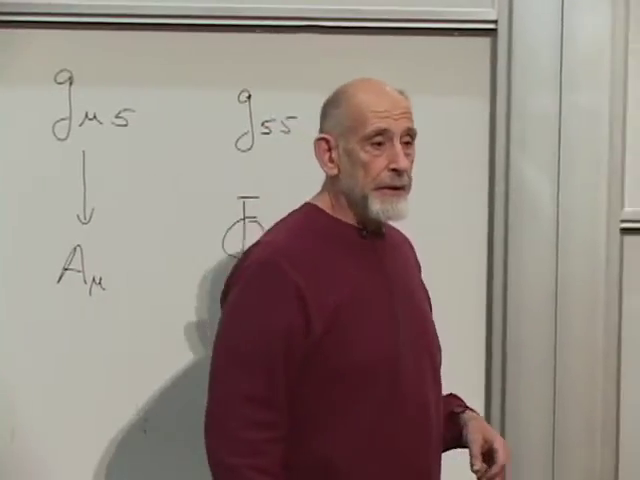
\includegraphics[width=0.72\textwidth]{lecture_10_figure_04.png}
  \caption{板書上的緊緻方向動量量子數。本講以示意方式將動量寫成緊緻方向速度的積分。}
  \lectureframe{00:21:30}
  \label{fig:l10-compact-momentum-board}
\end{figure}

纏繞 \(|w|\) 次的弦，其長度為 \(2\pi |w|R\)。基本弦張力為
\begin{equation}
  T_{\rm F}=\frac{1}{2\pi\alpha'},
\end{equation}
因此纏繞能量為
\begin{equation}
  E_{\rm wind}=T_{\rm F}(2\pi |w|R)
  =\frac{|w|R}{\alpha'}.
  \label{eq:l10-winding-energy}
\end{equation}
在本講採用的單位 \(\alpha'=1\) 下，能量就是 \(E_{\rm wind}=|w|R\)。

半徑變化時，兩座能譜塔的行為恰好相反。當 \(R\gg
\sqrt{\alpha'}\) 時，動量能級間距小，纏繞能級間距大。當 \(R\ll\sqrt{\alpha'}\) 時，動量能級間距大，纏繞能級間距小。

\begin{figure}[H]
  \centering
  \begin{minipage}[t]{0.48\textwidth}
    \centering
    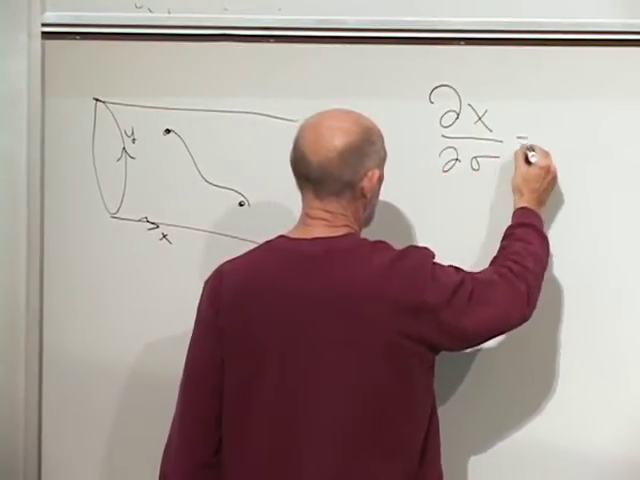
\includegraphics[width=\linewidth]{lecture_10_figure_05.png}
    \par\smallskip
    \textit{緊緻半徑較大。}
  \end{minipage}\hfill
  \begin{minipage}[t]{0.48\textwidth}
    \centering
    \includegraphics[width=\linewidth]{lecture_10_figure_06.png}
    \par\smallskip
    \textit{緊緻半徑較小。}
  \end{minipage}
  \caption{板書比較的兩種能譜。半徑取倒數後，稀疏與密集的能譜塔互換角色。}
  \lectureframe{00:25:30--00:26:00}
  \label{fig:l10-dual-spectra-board}
\end{figure}

清楚的示意圖如下
\begin{figure}[H]
  \centering
  \begin{adjustbox}{max width=\linewidth}
  \begin{tikzpicture}[x=1cm,y=0.74cm,>=Latex]
    \node[font=\bfseries] at (-3.6,6.2) {$R\gg\sqrt{\alpha'}$};
    \draw[->] (-5.1,0) -- (-5.1,5.5) node[above] {$E$};
    \foreach \y in {0.4,1.0,1.6,2.2,2.8,3.4,4.0,4.6}
      \draw (-5.35,\y)--(-4.85,\y);
    \node[align=center] at (-4.25,5.15) {momentum\\dense};
    \draw[->] (-2.2,0) -- (-2.2,5.5) node[above] {$E$};
    \foreach \y in {0.4,2.4,4.4}
      \draw (-2.45,\y)--(-1.95,\y);
    \node[align=center] at (-1.35,5.15) {winding\\sparse};

    \node[font=\bfseries] at (3.6,6.2) {$R\ll\sqrt{\alpha'}$};
    \draw[->] (2.2,0) -- (2.2,5.5) node[above] {$E$};
    \foreach \y in {0.4,2.4,4.4}
      \draw (1.95,\y)--(2.45,\y);
    \node[align=center] at (3.05,5.15) {momentum\\sparse};
    \draw[->] (5.1,0) -- (5.1,5.5) node[above] {$E$};
    \foreach \y in {0.4,1.0,1.6,2.2,2.8,3.4,4.0,4.6}
      \draw (4.85,\y)--(5.35,\y);
    \node[align=center] at (5.95,5.15) {winding\\dense};
  \end{tikzpicture}
  \end{adjustbox}
  \caption{能級間距論證的重建。動量與纏繞數連同 \(R\leftrightarrow\alpha'/R\) 一起互換時，完整的弦譜保持不變。}
  \label{fig:l10-dual-spectra-redraw}
\end{figure}

假設有人拿到其中一種能譜，卻不知道它是如何形成的。間距較小的能譜塔，究竟代表大圓上的動量，還是小圓上的纏繞？單憑能譜無法判斷。弦理論提出更強的主張：散射振幅也無法判別這兩種描述。它們在
\begin{equation}
  n\longleftrightarrow w,
  \qquad
  R\longleftrightarrow \widetilde R=\frac{\alpha'}{R}.
  \label{eq:l10-radius-duality}
\end{equation}
之下完全等價。自對偶半徑為
\begin{equation}
  R=\sqrt{\alpha'},
  \label{eq:l10-self-dual-radius}
\end{equation}
也就是本講單位下的 \(R=1\)。在這個半徑處，額外的態可能變成無質量態，規範對稱性也會增強。

\begin{classroomqa}
\audiencequestion{纏繞只是一種重寫能譜的數學技巧嗎？\lecturetimestamp{00:27:33}}
\lecturerresponse{不是。纏繞標記閉弦希爾伯特空間中的真實扇區，而這些扇區也參與交互作用。``對偶''意指動量描述與纏繞描述是同一物理的不同座標，而不是其中一個扇區只是另一個扇區可有可無的助記方式。}
\end{classroomqa}

\begin{classroomqa}
\audiencequestion{是否有一個半徑在對偶作用下映射到自身？
\lecturetimestamp{00:27:58}}
\lecturerresponse{有。自對偶半徑為 \(R=\sqrt{\alpha'}\)，以板書採用的單位表示則是 \(R=1\)。兩座能譜塔在此相遇，能譜也具有增強的對稱性。}
\end{classroomqa}

\section{對偶性的世界面表述}

能譜的論證頗具啟發性，但世界面上的描述能更精確地說明這種交換。在共形規範下，與 \(Y\) 共軛的動量正比於 \(\partial_\tau Y\)。因此，總緊緻方向動量的形式為
\begin{equation}
  P_Y=\frac{1}{2\pi\alpha'}
      \int_0^{2\pi}d\sigma\,\partial_\tau Y.
  \label{eq:l10-worldsheet-momentum}
\end{equation}
纏繞數則為
\begin{equation}
  w=\frac{1}{2\pi R}
      \int_0^{2\pi}d\sigma\,\partial_\sigma Y
   =\frac{Y(2\pi)-Y(0)}{2\pi R}.
  \label{eq:l10-worldsheet-winding}
\end{equation}

\begin{classroomqa}
\audiencequestion{為什麼沿閉弦積分導數不會得到零？\lecturetimestamp{00:32:33}}
\lecturerresponse{因為 \(Y\) 是週期性的靶空間座標，並非定義在 \(\sigma\) 圓上的單值實函數。世界面上的點 \(\sigma=2\pi\) 與 \(\sigma=0\) 是同一點，但將嵌入映射提升到覆蓋直線後，座標會改變 \(2\pi wR\)。對 \(\partial_\sigma Y\) 積分量度的正是這個位移。}
\end{classroomqa}

\begin{figure}[H]
  \centering
  \includegraphics[width=0.76\textwidth]{lecture_10_figure_07.png}
  \caption{板書完成兩行推導後得到的動量與纏繞數積分。本講採用的規範化略去了共同因子 \(2\pi\) 與 \(\alpha'\)。}
  \lectureframe{00:33:25}
  \label{fig:l10-momentum-winding-integrals}
\end{figure}

對於纏繞一圈的弦，
\begin{equation}
  Y(\tau,\sigma+2\pi)=Y(\tau,\sigma)+2\pi R.
\end{equation}
纏繞數為 \(w\) 時，右側的位移為 \(2\pi wR\)。因此，方程式 \eqref{eq:l10-worldsheet-winding} 會精確計數纏繞數。這是板書簡寫 \(w\sim R^{-1}\int
d\sigma\,\partial_\sigma Y\) 的精確表述。

因此，T 對偶在世界面上的表述為
\begin{equation}
  \partial_\tau Y\longleftrightarrow
  \partial_\sigma \widetilde Y,
  \qquad
  \partial_\sigma Y\longleftrightarrow
  \partial_\tau \widetilde Y,
  \label{eq:l10-derivative-duality}
\end{equation}
也就是說，\(Y\) 中的動量會變成對偶座標 \(\widetilde Y\) 中的纏繞，反之亦然。

\begin{classroomqa}
\audiencequestion{這是否表示世界面座標 \(\tau\) 和 \(\sigma\) 本身彼此相關或互換？
\lecturetimestamp{00:34:39}}
\lecturerresponse{不是。T 對偶會映射解，並交換緊緻靶空間座標的特定導數；它不會把世界面的時間座標與空間座標視為相同。}
\end{classroomqa}

\section{為什麼無法排除纏繞態}

有人或許會問：既然弦也可以處於未纏繞態，為什麼還會出現纏繞態？弦不會依照偏好選擇狀態。碰撞所提供的能量會拉伸弦。能量足夠高、形變嚴重的弦，可能重新接合成兩根纏繞方向相反的弦。它們的總纏繞數仍為零，但分裂後兩根弦可能彼此分離。若將其中一根送到很遠的地方，觀察者便會看到一根似乎孤立的纏繞弦。

\begin{figure}[H]
  \centering
  \includegraphics[width=0.76\textwidth]{lecture_10_figure_08.png}
  \caption{淨纏繞數為零且高度拉伸的組態；重新接合後，纏繞方向相反的弦可以由此分離。}
  \lectureframe{00:36:15}
  \label{fig:l10-winding-pair-production}
\end{figure}

能量閾值由纏繞能量決定。在大圓上，必須有很高的碰撞能量，才能將足夠長的弦沿緊緻方向拉伸。然而，能量一旦超過閾值，纏繞--反纏繞對的產生便無法禁止。這類似光子碰撞產生電子--正電子對。總電荷仍為零，但帶電粒子確實存在，而且可以彼此分離。纏繞數守恆也以相同方式運作。

這個類比不只是說法相似。緊緻方向動量與纏繞是兩種不同的荷量子數。在相應的約化描述中，同號相斥、異號相吸。因此，我們應該找出傳遞這兩種作用力的向量場。

\section{五維引力中的動量荷}

從五維引力開始。大寫指標 \(M,N\) 遍歷四個普通時空方向和緊緻的第五方向。度規分解如下：
\begin{equation}
  G_{MN}\quad\longrightarrow\quad
  \bigl\{G_{\mu\nu},\,G_{\mu5},\,G_{55}\bigr\}.
  \label{eq:l10-metric-decomposition}
\end{equation}
對稱分量 \(G_{5\mu}\) 不包含 \(G_{\mu5}\) 以外的新資訊。

\begin{figure}[H]
  \centering
  \includegraphics[width=0.74\textwidth]{lecture_10_figure_09.png}
  \caption{五維度規分量的獨立群組：\(G_{\mu\nu}\)、\(G_{\mu5}\) 與 \(G_{55}\)。}
  \lectureframe{00:44:05}
  \label{fig:l10-metric-components}
\end{figure}

從四維觀點來看，
\begin{align}
  G_{\mu\nu} &\quad\hbox{is a spacetime metric},\\
  G_{\mu5} &\equiv A_\mu\quad\hbox{is a vector field},\\
  G_{55} &\equiv e^{2\varphi}\quad\hbox{is a scalar modulus}.
  \label{eq:l10-four-dimensional-fields}
\end{align}
標量 \(\varphi\) 量度緊緻方向的尺度。它可以在普通時空中平滑變化，因此 \(\varphi\) 的波就是第五維半徑的波動。

\begin{figure}[H]
  \centering
  \includegraphics[width=0.74\textwidth]{lecture_10_figure_10.png}
  \caption{板書將 \(G_{\mu5}\) 對應為向量 \(A_\mu\)，並將 \(G_{55}\) 對應為標量 \(\Phi\)。}
  \lectureframe{00:47:40}
  \label{fig:l10-vector-and-radius-modulus}
\end{figure}

混合引力分量的來源是混合動量流。具體而言，沿第五方向的動量會成為 \(G_{\mu5}\) 的源。因此，四維觀察者會將整數 \(n\) 解讀為與 \(A_\mu\) 耦合的電荷。這就是 Kaluza--Klein 機制：在高維幾何中表現為動量的量，在低維場論中則成為電荷。

\editorialnote{本講將來自 \(G_{55}\) 的標量概略地稱為``膨脹子''。在這種約化中，它實際上是半徑模量。控制弦耦合的十維弦膨脹子是另一個場，不過改變標架或施行對偶時，低維的標量組合可能會彼此混合。}

\begin{classroomqa}
\audiencequestion{標量 \(\varphi\) 是否正比於動量整數 \(n\)？\lecturetimestamp{00:48:43}}
\lecturerresponse{不是。整數 \(n\) 標記一個量子化態，並作為電荷。標量 \(\varphi(x)\) 是決定局部緊緻化尺度的連續場。它可以隨位置改變，本身並不是整數。}
\end{classroomqa}

\section{第二個向量場與纏繞荷}

纏繞也具有類似電荷的性質，但它不能以相同方式耦合到同一個向量場。要找出第二個向量場，可以回頭看最初的閉弦激發。閉弦有左行與右行振子模態。物理態必須滿足能級匹配條件：左行與右行的總激發能級必須相同。

在玻色弦理論中，未激發態是快子。只含一個左行或右行振子的態不符合能級匹配條件。因此，第一個允許的無質量態必須同時包含兩種振子，各一個：
\begin{equation}
  \alpha_{-1}^{I}\widetilde\alpha_{-1}^{J}\ket{0;k}.
  \label{eq:l10-first-massless-state}
\end{equation}
指標 \(I,J\) 遍歷橫向空間方向，包括緊緻方向。若一個指標對應普通方向，另一個則是 \(5\)，便會有兩種類似向量的振子態：
\begin{equation}
  \alpha_{-1}^{\mu}\widetilde\alpha_{-1}^{5}\ket{0;k},
  \qquad
  \alpha_{-1}^{5}\widetilde\alpha_{-1}^{\mu}\ket{0;k}.
  \label{eq:l10-two-vector-states}
\end{equation}

\begin{figure}[H]
  \centering
  \includegraphics[width=0.76\textwidth]{lecture_10_figure_11.png}
  \caption{當其中一個極化方向沿著緊緻方向時，兩種左--右振子排列會形成四維向量態。}
  \lectureframe{00:58:20}
  \label{fig:l10-two-vector-states-board}
\end{figure}

它們的對稱組合與反對稱組合分別屬於不同的時空場：
\begin{align}
  \alpha_{-1}^{(\mu}\widetilde\alpha_{-1}^{5)}\ket{0;k}
    &\longleftrightarrow G_{\mu5},\\
  \alpha_{-1}^{[\mu}\widetilde\alpha_{-1}^{5]}\ket{0;k}
    &\longleftrightarrow B_{\mu5}.
  \label{eq:l10-g-and-b-vectors}
\end{align}
前者是以緊緻動量為源的 Kaluza--Klein 向量。後者源自反對稱的 Kalb--Ramond 場，並以弦纏繞為源。因此，約化後的理論包含兩個類似光子的場，分別對應兩種荷扇區。

若兩個振子指標都指向緊緻方向，該態就是與緊緻化模量相關的標量。若兩者都指向普通的橫向方向，對稱無跡部分就是引力子，反對稱部分是 \(B_{\mu\nu}\)，而跡則對應一個標量扇區。

\begin{classroomqa}
\audiencequestion{這些態中，哪個是單態，哪個是三重態？\lecturetimestamp{01:00:21}}
\lecturerresponse{在此採用這種分類並無助益。兩種混合態都以四維向量的形式變換。將它們相加與相減，可以分離出對稱的度規極化與反對稱的 \(B\) 場極化。具有兩個緊緻方向指標的態則是四維標量。}
\end{classroomqa}

休息前整理出的完整對應關係如下：
\begin{equation}
  \boxed{
  \begin{gathered}
    n\leftrightarrow w,
    \qquad
    R\leftrightarrow\dfrac{\alpha'}{R},\\
    \partial_\tau Y\leftrightarrow\partial_\sigma\widetilde Y,
    \qquad
    G_{\mu5}\leftrightarrow B_{\mu5}.
  \end{gathered}}
  \label{eq:l10-complete-t-duality-map}
\end{equation}

\begin{figure}[H]
  \centering
  \includegraphics[width=0.72\textwidth]{lecture_10_figure_12.png}
  \caption{板書總結了 T 對偶的對應關係：動量與纏繞、半徑與倒數半徑、世界面導數，以及兩個向量場都會互換。講者將最後一行部分遮住，因此我們在方程式 \eqref{eq:l10-complete-t-duality-map} 中明確列出該行。}
  \lectureframe{01:02:20}
  \label{fig:l10-t-duality-map-board}
\end{figure}

不應將這項構造誤解為：上述每個場都已在觀測到的粒子譜中找到對應粒子。就目前而言，這只是緊緻化弦理論的一項數學結果。雖然有許多方案嘗試將這些結構與現象學連結起來，但這不是本講要處理的問題。

\section{開弦帶來新的問題}

休息後，我們重新從開弦談起。閉弦沒有端點，纏繞便無法從端點滑脫，因此可以穩定地纏繞。開弦有端點，因而沒有類似的拓撲保護纏繞數。然而，T 對偶是理論的精確對稱性。這項對稱性會如何作用於開弦？

對於自由運動的端點，弦作用量的變分會導出 Neumann 邊界條件。在簡單的 \((X,Y)\) 幾何中，
\begin{equation}
  \left.\partial_\sigma X\right|_{\partial\Sigma}=0,
  \qquad
  \left.\partial_\sigma Y\right|_{\partial\Sigma}=0.
  \label{eq:l10-neumann-boundary}
\end{equation}
力學圖像很直觀。把弦視為由無數個愈來愈小的質量元串成的鏈。若末端質量元受到非零的切向力，當它的質量趨近於零時，加速度便會發散。因此，自由端點會自行調整，直到端點的合張力為零。也可以由人固定端點並施加所需的力，但如此一來，端點便不再是自由的。

\begin{figure}[H]
  \centering
  \includegraphics[width=0.76\textwidth]{lecture_10_figure_13.png}
  \caption{開弦及其完整的 Neumann 端點條件：\(\partial_\sigma X=\partial_\sigma Y=0\)。}
  \lectureframe{01:09:20}
  \label{fig:l10-neumann-board}
\end{figure}

現在只對緊緻座標 \(Y\) 施行對偶變換。非緊緻座標 \(X\) 保持不變。方程式 \eqref{eq:l10-derivative-duality} 會將第二個 Neumann 條件轉換為
\begin{equation}
  \left.\partial_\tau\widetilde Y\right|_{\partial\Sigma}=0.
  \label{eq:l10-dirichlet-time-derivative}
\end{equation}
因此，端點在對偶緊緻方向上的位置不隨時間改變：
\begin{equation}
  \left.\widetilde Y\right|_{\partial\Sigma}=Y_0.
  \label{eq:l10-dirichlet-boundary}
\end{equation}
這就是 Dirichlet 邊界條件。

\begin{figure}[H]
  \centering
  \includegraphics[width=0.76\textwidth]{lecture_10_figure_14.png}
  \medskip

  \begin{adjustbox}{max width=\linewidth}
  \begin{tikzpicture}[x=1cm,y=1cm,>=Latex]
    \node[align=center] at (-3.5,0.8)
      {Neumann\\\(\left.\partial_\sigma Y\right|_{\partial\Sigma}=0\)};
    \draw[->,thick] (-1.7,0.8) -- (1.3,0.8)
      node[midway,above] {$T_Y$};
    \node[align=center] at (3.4,0.8)
      {Dirichlet\\\(\left.\partial_\tau\widetilde Y\right|_{\partial\Sigma}=0\)};
    \node[align=center] at (3.4,-0.5)
      {\(\widetilde Y(\tau)=Y_0\) at each endpoint};
  \end{tikzpicture}
  \end{adjustbox}
  \caption{板書上已完成的對偶端點條件，以及對其邏輯的清楚重建。T 對偶會將緊緻方向上的自由運動轉換為端點在對偶方向上的固定位置。}
  \lectureframe{01:12:35}
  \label{fig:l10-neumann-to-dirichlet}
\end{figure}

\begin{classroomqa}
\audiencequestion{為什麼對偶條件表示端點是固定的？\lecturetimestamp{01:12:39}}
\lecturerresponse{因為 \(\partial_\tau\widetilde Y=0\) 表示端點在對偶方向上的速度為零。無論端點起初位於 \(\widetilde Y\) 的哪個位置，它都會停留在該處。端點沿未施行對偶變換之方向的座標仍可自由變動。}
\end{classroomqa}

\section{固定端點的物體是 D 膜}

若端點固定，就必須有某種物體能將它留在原處。因此，精確的 T 對偶要求理論中存在一種可供開弦終止其上的新物體，也就是 D 膜。字母 \(D\) 代表 Dirichlet，並非該物體的維度。講座中提到一段歷史掌故：這些物體或許可以 Joseph Polchinski 命名，因為他的分析明確揭示了它們的動力學角色；不過，既有術語``p 膜''使 Dirichlet 成為自然的名稱。

一個 \(p\) 膜有 \(p\) 個空間維度。弦是一膜，膜是二膜，延展的三維物體則是三膜。D\(p\) 膜是一種 \(p\) 膜，基本弦端點在垂直於膜的方向上滿足 Dirichlet 條件，在沿著膜的方向上則滿足 Neumann 條件。

對偶論證並未指定 \(Y_0\) 的特定值，因此 D 膜不可能是釘在宇宙某個特定位置上的剛性固定物。它必須能夠移動。相對論也不允許絕對剛性的延展物體，因此 D 膜可以振動、彎曲。板書畫出的平坦膜只是其平衡組態，並非對其動力學的限制。

\begin{classroomqa}
\audiencequestion{開弦的兩個端點必須位於對偶座標相同的固定位置嗎？\lecturetimestamp{01:14:55}}
\lecturerresponse{不一定。兩個端點可以位於同一張 D 膜上，此時它們共享該膜在垂直方向上的位置；也可以分別位於兩張位置不同的 D 膜上，弦便會在兩膜之間伸展。膜本身也可能振動、彎曲，因此端點所在的軌跡不必始終是完全平坦的平面。}
\end{classroomqa}

\section{計算 D 膜的維度}

十維超弦理論有九個空間維度。假設 T 對偶在一個空間方向上施加 Dirichlet 條件，端點在其餘八個方向上仍可自由移動，因此其允許所在的位置構成一張八維 D8 膜。每增加一個獨立的 Dirichlet 條件，端點可移動的方向便少一個。若有 \(k\) 個空間座標被固定，則
\begin{equation}
  p=9-k.
  \label{eq:l10-dp-counting}
\end{equation}

桌面提供了同一種維度計數的三維例子。固定垂直座標後，指尖仍可在二維桌面上移動；再固定一個座標後，指尖便只能沿著一條線移動；三個座標全都固定時，指尖就被限制在一個點上。

\begin{figure}[H]
  \centering
  \begin{adjustbox}{max width=\linewidth}
  \begin{tikzpicture}[x=1.05cm,y=1cm,>=Latex]
    \draw[fill=blue!8] (-5.5,-0.7) -- (-2.5,-0.7) -- (-1.7,0.2)
      -- (-4.7,0.2) -- cycle;
    \node at (-3.6,-1.15) {one constraint: sheet};
    \draw[very thick,blue!60!black] (-0.9,-0.25) -- (1.3,-0.25);
    \node at (0.2,-1.15) {two constraints: line};
    \fill[blue!70!black] (4.1,-0.25) circle (0.09);
    \node at (4.1,-1.15) {three constraints: point};
    \draw[->] (-1.45,0.95) -- (-0.75,0.95);
    \draw[->] (2.25,0.95) -- (2.95,0.95);
    \node at (0.35,1.35) {each Dirichlet condition lowers \(p\) by one};
  \end{tikzpicture}
  \end{adjustbox}
  \caption{在桌面上說明維度計數的論證。D\(p\) 膜是端點仍能自由移動的所在位置。}
  \label{fig:l10-dp-counting-redraw}
\end{figure}

反覆施行對偶變換，可以生成 D8 膜、D7 膜、D6 膜，依此類推，直到空間中呈點狀的 D0 膜。若沒有任何空間方向受到固定，D9 膜便遍布全部九個空間維度，普通開弦也能在各處自由移動。講座中簡短提到 D\((-1)\) 膜；這類膜局域於歐幾里得時空中，表現為瞬子，而非隨時間傳播的普通粒子。

\editorialnote{這個維度階梯描述的是合併來看時的 II 型理論。穩定的 BPS D\(p\) 膜在 IIA 型理論中具有偶數個 \(p\)，在 IIB 型理論中則具有奇數個 \(p\)。沿一個圓施行 T 對偶會使 \(p\) 改變一，並同時將 IIA 型與 IIB 型理論互換。}

\begin{classroomqa}
\audiencequestion{如果只有六個維度是緊緻的，計算維度時是否應該從六開始扣除，而不是從九開始？\lecturetimestamp{01:20:49}}
\lecturerresponse{這個基本推導是在緊緻方向上施行 T 對偶；當原本的圓縮到任意小時，其對偶圓便會擴大到任意大。在這個極限下，對偶圓實際上成為非緊緻方向。因此，所得的膜可以沿著在可及尺度下看似非緊緻的方向延伸，也可以垂直於這類方向。維度 \(p\) 計算的是沿著膜的所有空間方向，而不只是在某項推導中使用的緊緻方向。}
\end{classroomqa}

D0 膜是一種新型粒子。開弦可以從一張 D0 膜延伸至另一張 D0 膜，可以返回同一張 D 膜，也可以朝非常遙遠的膜延伸。若弦真的延伸到空間無窮遠處，其長度便是無限大，能量也因此無限大；所以在物理上有用的情況，是讓弦的另一端連接到另一個物體上。

下一個情形是 D1-膜。它本身具有弦狀，但不是我們一開始討論的基本弦。它可以彎曲，也可以閉合成環；基本弦則可以終止於其上。它的張力隨弦耦合常數變化的方式不同：
\begin{equation}
  T_{\rm D1}=\frac{1}{2\pi\alpha' g_s},
  \qquad
  T_{\rm F1}=\frac{1}{2\pi\alpha'}.
  \label{eq:l10-dstring-tension}
\end{equation}
在弱耦合 \(g_s\ll1\) 下，D 弦比基本弦重得多，這也解釋了它為何一開始會像一個質量很大的錨。

\begin{figure}[H]
  \centering
  \includegraphics[width=0.76\textwidth]{lecture_10_figure_15.png}
  \caption{黑板上的 D1-膜：一種可彎曲的一維物體，與可終止於其上的基本弦不同。}
  \lectureframe{01:24:20}
  \label{fig:l10-d1-brane}
\end{figure}

\begin{classroomqa}
\audiencequestion{T 對偶也作用於 D 膜嗎？\lecturetimestamp{01:25:35}}
\lecturerresponse{會。沿著 D\(p\)-膜平行方向進行 T 對偶，會使其維度降為 D\((p-1)\)；沿著垂直方向進行 T 對偶，則會使其維度升為 D\((p+1)\)。膜也是對偶對應的一部分，並非在對偶作用下保持不變的外部支撐物。}
\end{classroomqa}

\begin{classroomqa}
\audiencequestion{沿著膜的方向仍然可以是緊緻的嗎？
\lecturetimestamp{01:27:25}}
\lecturerresponse{可以。``沿膜方向''與``緊緻''回答的是不同問題。一個方向可以沿著膜，同時閉合成圓；也可以是非緊緻的。對端點而言，關鍵在於該方向上的邊界條件是諾伊曼型還是狄利克雷型。}
\end{classroomqa}

D2-膜是一張類似薄片的膜。D3-膜有三個空間維度。在真正的高維時空中，D3-膜是三維子空間，而非整個空間；即使受限於膜上的觀測者，仍可能將它視為自身完整的空間世界。

\begin{figure}[H]
  \centering
  \includegraphics[width=0.76\textwidth]{lecture_10_figure_16.png}
  \caption{畫成薄片的 D2-膜，弦端點可以在其上移動。}
  \lectureframe{01:27:55}
  \label{fig:l10-d2-brane}
\end{figure}

這裡給出的推導刻意只作概略說明。單憑它本身，還不能證明弦理論描述了自然界。然而，在弦理論內部，有許多一致性檢驗：對偶性、量子計算和數學結果都指向 D 膜是真正的動力學物體。

\section{膜上的開弦成為場}

取一張除此之外空無一物的 D2-膜，並在其上放置短開弦。每個端點都受限於膜面，因此整個低能激發會沿著膜面移動。兩條有向弦若相鄰端點的箭頭相容，就可以接合；接合後的弦之後還可以再次分裂。若將這些過程視為粒子歷史，它們就是費曼圖的頂點：兩個粒子進入，中間有一個激發傳播，接著兩個粒子出來。

\begin{figure}[H]
  \centering
  \includegraphics[width=0.76\textwidth]{lecture_10_figure_17.png}
  \caption{D2-膜上的有向開弦透過相容的端點接合。在低能下，這個過程可視為膜上的場論交互作用。}
  \lectureframe{01:29:55}
  \label{fig:l10-open-strings-on-brane}
\end{figure}

在遠低於弦尺度的能量下，內部振動譜塔不會被激發。剩下的無質量開弦態，是膜世界體上的向量場。對單張膜而言，這是阿貝爾 \(U(1)\) 規範場，相當於膜上的電磁場。這個場不會在整個十維體空間中傳播；它的量子是開弦，而弦的端點使它們受限於膜上。

\section{膜堆疊產生非阿貝爾色荷}

現在把數張平行膜放在彼此附近。以三張膜為例，分別標記為紅、綠、藍。一條有向弦的兩個端點各有一個標籤，且標籤有序：例如，它可以從紅膜延伸到綠膜、從綠膜延伸到藍膜，或從紅膜延伸回紅膜。對於 \(N\) 張膜，無質量開弦態可以排列成一個 \(N\times N\) 矩陣：
\begin{equation}
  A_\mu{}^{i}{}_{j},
  \qquad i,j=1,\ldots,N.
  \label{eq:l10-chan-paton-matrix}
\end{equation}
這些就是 --Chan–Paton 標籤，對應一個 \(U(N)\) 規範理論。

\begin{figure}[H]
  \centering
  \includegraphics[width=0.76\textwidth]{lecture_10_figure_18.png}
  \medskip

  \begin{adjustbox}{max width=\linewidth}
  \begin{tikzpicture}[x=1cm,y=1cm,>=Latex]
    \draw[very thick,red!70!black] (-4.8,2.0)--(4.8,2.0);
    \draw[very thick,green!55!black] (-4.8,0.8)--(4.8,0.8);
    \draw[very thick,blue!70!black] (-4.8,-0.4)--(4.8,-0.4);
    \node[left] at (-4.8,2.0) {Red};
    \node[left] at (-4.8,0.8) {Green};
    \node[left] at (-4.8,-0.4) {Blue};
    \draw[->,thick] (-3.4,2.0) .. controls (-2.8,1.35) and (-2.3,1.15)
      .. (-1.7,0.8);
    \node at (-2.7,1.05) {$R\!G$};
    \draw[->,thick] (-0.6,0.8) .. controls (0.0,0.25) and (0.6,-0.05)
      .. (1.2,-0.4);
    \node at (0.1,0.0) {$G\!B$};
    \draw[->,thick] (2.1,2.0) .. controls (2.9,2.55) and (3.8,2.55)
      .. (4.3,2.0);
    \node at (3.2,2.65) {$R\!R$};
  \end{tikzpicture}
  \end{adjustbox}
  \caption{黑板上的三張平行膜，以及對膜間弦所帶有序端點標籤的清楚重構。}
  \lectureframe{01:33:15}
  \label{fig:l10-three-brane-stack}
\end{figure}

\begin{classroomqa}
\audiencequestion{一條弦真的能從紅膜延伸到綠膜，而不被其他圖線擋住嗎？\lecturetimestamp{01:35:07}}
\lecturerresponse{可以。這些膜嵌入更高維空間中。黑板上的二維圖像只是投影，因此弦可以沿著垂直於投影面的方向，繞過另一條投影線。}
\end{classroomqa}

\begin{classroomqa}
\audiencequestion{紅--綠弦必須與綠--藍弦接合，才能成為紅--藍弦嗎？\lecturetimestamp{01:35:39}}
\lecturerresponse{這是基本的局部接合規則。相容的端點相遇後，兩段弦接合成一條弦，未接合的端點則保留紅、藍標籤。更複雜的過程可以透過重複相同的操作構成。}
\end{classroomqa}

接合規則就是幾何化的矩陣乘法。紅--綠弦可以與綠--藍弦接合，因為兩條弦的綠色端點彼此相容。結果是一條紅--藍弦：
\begin{equation}
  (R,G)\circ(G,B)\longrightarrow(R,B).
  \label{eq:l10-color-composition}
\end{equation}
重複出現的指標在接合處相連，並在內部消去。這與 Yang--–Mills 交互作用頂點上的指標結構相同。

\begin{figure}[H]
  \centering
  \includegraphics[width=0.76\textwidth]{lecture_10_figure_19.png}
  \caption{堆疊膜上的開弦接合。端點取向確保其組合方式與非阿貝爾規範場採用的有序指標組合相同。}
  \lectureframe{01:36:30}
  \label{fig:l10-color-joining-board}
\end{figure}

對於三張重合的膜，完整的開弦規範群是 \(U(3)\)，共有九種向量態。其代數可分解為
\begin{equation}
  \mathfrak u(3)=\mathfrak{su}(3)\oplus\mathfrak u(1).
  \label{eq:l10-u3-decomposition}
\end{equation}
八個無跡組合具有 QCD 膠子的色結構，而對角的質心 \(U(1)\) 則是另一個獨立的阿貝爾場。

\editorialnote{講座把九種色對組合中的一種描述成可以脫離並消失，於是留下八個膠子。精確地說，三張重合膜組成的堆疊給出 \(U(3)\)，而不只是 \(SU(3)\)。要得到 QCD 八重態，必須分離、投影掉或以其他方式解耦對角的 \(U(1)\)。講座中的圖像確實有助於理解有序色指標，但並未完整推導出 QCD。}

類夸克物質只帶有一個色指標。在膜的圖像中，它由一條弦表示，弦的一個端點位於色膜堆疊上，另一個端點則位於另一張遙遠的膜上。相對於色膜堆疊而言，只有一端顯示出色標籤。反轉弦的取向，就得到反粒子。若一條類夸克弦與一條類反夸克弦的端點相容，兩者便可以接合並離開色膜堆疊；兩條取向相同的類夸克弦則無法以這種方式湮滅。

由此得到的低能理論通常是超對稱 Yang--–Mills 理論，附加物質則由膜及其交會方式決定。這些理論與 QCD 足夠相近，能用來闡明非阿貝爾動力學，但不會自動成為標準模型。若只有一張膜，相同的構造便化約為 \(U(1)\) 理論：短的膜--膜弦類似光子，而延伸至另一個扇區的有向弦則扮演正、負電荷的角色。

\section{D 弦終止於磁單極子}

現在的圖像中有兩種弦狀物體。原先的基本弦，也就是 F 弦，在 D3-膜上承載電通量。D1-膜，也就是 D 弦，在弱耦合下重得多。D 弦也可以終止於 D3-膜上。它的端點對世界體規範場而言不帶電，但帶有磁荷。對 D3-膜上的觀測者而言，這個端點就是磁單極子。

\begin{figure}[H]
  \centering
  \includegraphics[width=0.76\textwidth]{lecture_10_figure_20.png}
  \medskip

  \begin{adjustbox}{max width=\linewidth}
  \begin{tikzpicture}[x=1cm,y=1cm,>=Latex]
    \draw[fill=blue!7] (-3.8,-0.5)--(2.6,-0.5)--(3.6,0.35)--(-2.8,0.35)--cycle;
    \node at (2.25,-0.95) {D3-brane};
    \draw[very thick,red!70!black] (0.0,3.0)--(0.0,0.0);
    \fill[black] (0.0,0.0) circle (0.08);
    \node[right] at (0.15,2.1) {D-string};
    \foreach \a in {25,65,115,155} {
      \draw[->,blue!65!black] (0.0,0.0)--({1.25*cos(\a)},{0.65*sin(\a)});
    }
    \node[align=center] at (4.8,1.7) {magnetic flux\\on the D3 worldvolume};
    \draw[->] (3.7,1.35)--(1.05,0.45);
  \end{tikzpicture}
  \end{adjustbox}
  \caption{黑板上的端點構造及其清楚的物理解讀。一條終止於 D3-膜上的 D 弦，在世界體規範理論中呈現為磁單極子。}
  \lectureframe{01:41:30}
  \label{fig:l10-dstring-monopole}
\end{figure}

質量階層在定性上也符合預期。由於 D 弦張力帶有因子 \(1/g_s\)，在弱耦合下，其端點比一般電激發重得多。F 弦與 D 弦端點的電磁關係，是 IIB 型弦理論更廣泛對偶結構的一部分。

\begin{classroomqa}
\audiencequestion{D 弦的端點是中性的嗎？
\lecturetimestamp{01:42:19}}
\lecturerresponse{若以基本弦端點所帶的電荷來看，它是中性的，但並非完全不帶電。它帶有磁荷，因此是 D3-膜規範理論中的磁單極子。}
\end{classroomqa}

\section{這個構造主張了什麼，又沒有主張什麼}

從 T 對偶到膜的這段發展歷經數十年逐步建立，並非來自單一計算。一個最初為描述強子而提出的理論，後來成為量子重力的候選理論。接著，理論中的對偶性使 D 膜必須納入其譜中；而規範理論也以弦終止於膜上的低能動力學之姿再次出現。從這個意義上說，這門學科走了一個完整的循環。

D 膜及相關的對偶構造，已成為研究超對稱規範理論、強耦合系統，以及引力與場論之間關聯的有力工具。它們也透過規範／引力對偶，為流體和電漿模型帶來啟發。這些成果並不等於直接推導出觀測到的粒子譜。緊緻化幾何、膜組態、超對稱破缺及許多其他要素，仍須加以選定。

\begin{classroomqa}
\audiencequestion{由什麼決定要對偶化哪個緊緻維度？
\lecturetimestamp{01:44:59}}
\lecturerresponse{從數學上說，只要具備所需的對稱性，任何緊緻方向都可以進行對偶化，並可選擇最方便的描述方式。從物理上說，特定狀態中實現的膜取向與緊緻化資料，則由該狀態的歷史和動力學所決定。}
\end{classroomqa}

\begin{classroomqa}
\audiencequestion{磁單極子的構造是由哪種膜承載？
\lecturetimestamp{01:45:21}}
\lecturerresponse{規範理論所在的世界是一張 D3-膜。D 弦延伸至垂直方向，並終止於這張 D3-膜；它的端點就是膜上三個空間維度中所見的磁單極子。}
\end{classroomqa}

\begin{classroomqa}
\audiencequestion{D 弦也有取向嗎？
\lecturetimestamp{01:45:55}}
\lecturerresponse{有。反轉 D 弦的取向會使相應的電荷反號。兩種端點取向分別代表磁單極子與反磁單極子，正如基本弦端點的取向可以區分電荷正負。}
\end{classroomqa}

\begin{classroomqa}
\audiencequestion{這種簡單的環面圖像能解釋手徵粒子物理中的左--右不對稱嗎？
\lecturetimestamp{01:46:05}}
\lecturerresponse{單靠它本身不行。平坦環面對稱性太高。手徵譜需要更多結構，例如不對稱的膜交會、軌形投影，或緊緻化在合適的 Calabi--–Yau 幾何上。弦理論中確有產生手徵性的機制，但超出這個初等 T 對偶構造的範圍。}
\end{classroomqa}

我們追蹤了同一種對稱性的四種具體表現：譜的交換、世界面導數的交換、時空場的交換，最後是端點邊界條件的交換。最後一種表現最具決定性。它將數學上的等價性轉化為 D 膜的發現，也將開弦的動力學轉化為其世界體上的規範理論。到了這一步，用 Susskind 的話說，這場講座已耗盡它的時間、能量與動量。